\section*{Results}

This section presents the experimental outcomes under two complementary perspectives: (i) detailed ConvMixer behavior analysis, and (ii) controlled cross-model comparison under an identical training protocol with multi-seed reporting.

\subsection*{Dataset Setup}

The investigation was conducted using a Vietnamese speech command dataset comprising a total of 4,460 audio samples, classified into 13 distinct command classes. These classes encompass smart device control commands (e.g., \textit{bat\_den}, \textit{tat\_tv}, \textit{mo\_rem}—turn on light, turn off TV, open curtains) alongside an unknown category. The data was partitioned into three subsets using stratified splitting to ensure high class representativeness and balanced distribution: the Training set comprised 75\% (3,341 samples), the Validation set 15\% (665 samples), and the Test set 10\% (454 samples). All compared models shared this split and the same preprocessing pipeline, and were evaluated across five random seeds (42--46) for statistical robustness. All input audio files underwent rigorous preprocessing (VAD, denoising) and were standardized into fixed-size Mel-spectrogram features of (128, 32) dimensions.

\subsection*{Model Training Procedure}

The ConvMixer model was implemented with an intrinsic hidden dimension ($dim$) of 256 and a depth of 8 repeating ConvMixer blocks. This configuration resulted in a small total parameter count of 719,117, lightweight compared to many contemporary deep learning architectures. The same training protocol (loss, optimizer family, scheduler policy, augmentation policy, and stopping criteria) was applied to all benchmarked models to ensure controlled comparison. To enhance generalization capability and mitigate potential overfitting, data augmentation techniques were applied exclusively to the training set. These techniques included Time Masking, Frequency Masking (randomly masking up to 10\% of the dimension with 50\% probability each), and Time Stretching (altering speed between 80\% and 120\% with 50\% probability).

Training dynamics were monitored on the validation set under the shared 25-epoch budget, with Early Stopping (patience=5, $min\_delta=0.02$) and $ReduceLROnPlateau$ scheduling. In the current ConvMixer reference run (seed 42), the best checkpoint was obtained at epoch 24, with test accuracy 97.14\%, macro-F1 0.9716, weighted-F1 0.9714, test loss 0.1103, and training time 468.4 seconds.

\begin{figure}[htbp]
  \centering

  \begin{minipage}{0.48\textwidth}
    \centering
    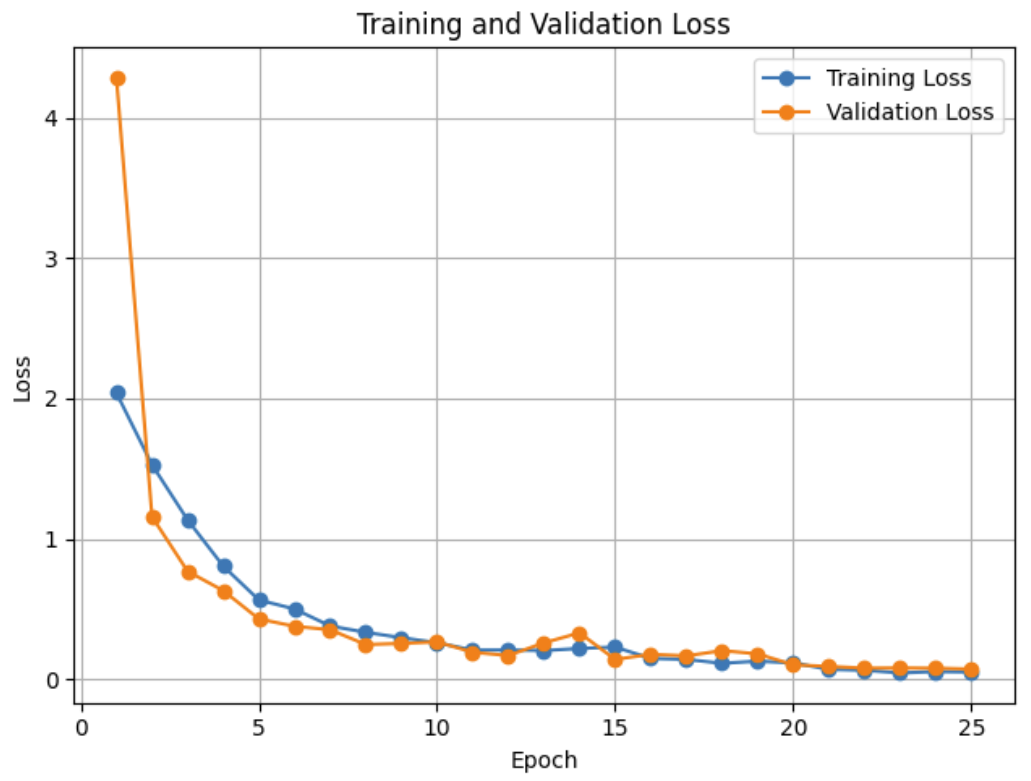
\includegraphics[width=\linewidth]{imgs/fig4.png}
    \caption*{(a) Training and validation loss}
  \end{minipage}\hfill
  \begin{minipage}{0.48\textwidth}
    \centering
    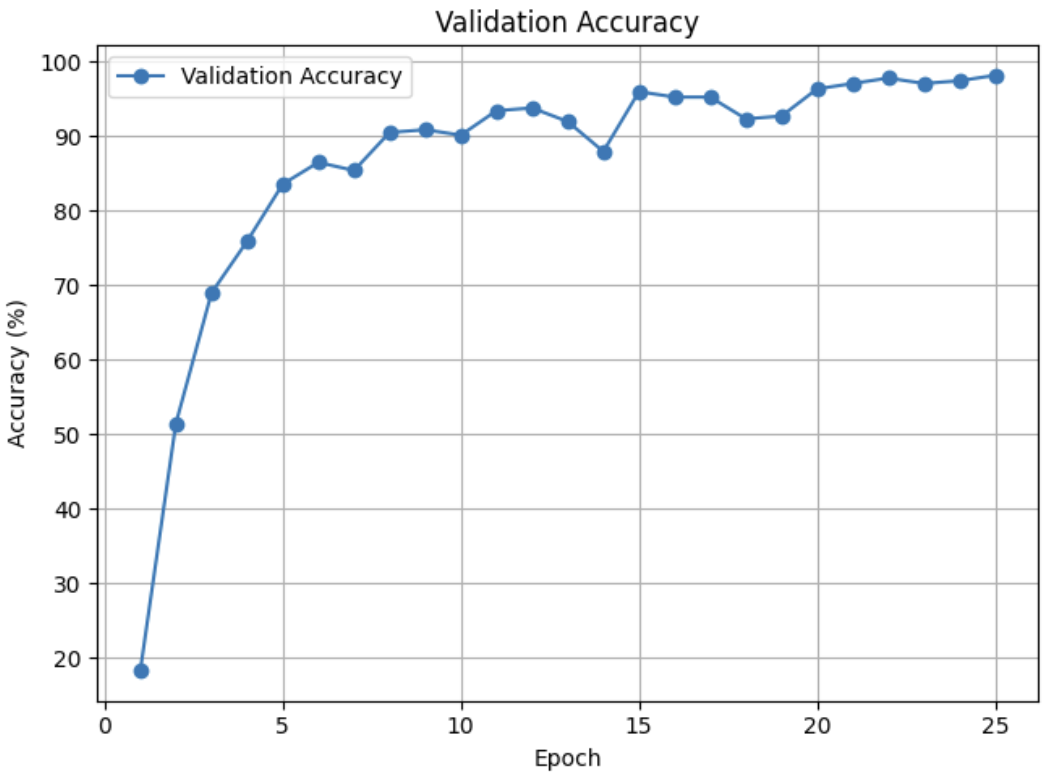
\includegraphics[width=\linewidth]{imgs/fig5.png}
    \caption*{(b) Validation accuracy}
  \end{minipage}

  \caption{
  Comparison of model performance across epochs. 
  (a) illustrates the convergence of training and validation loss, while 
  (b) shows the progression of validation accuracy
  }
  \label{fig:training_metrics}
\end{figure}

\subsection*{Controlled Multi-model Comparison (Five Seeds)}

Following reviewer recommendations, we established an aligned benchmark using five architectures trained on the same dataset and protocol: ConvMixer-256/8, ResNet-18, MobileNetV2, EfficientNet, and AST (tiny configuration). Each model was run with seeds 42--46, and the final report is presented as mean$\pm$std.

\begin{table}[htbp]
\centering
\small
\caption{\label{tab:controlled_model_comparison}Controlled model comparison on the Vietnamese speech command dataset. Accuracy/F1/Loss/Time are reported as mean$\pm$std over five seeds (42--46).}
\begin{tabular}{lcccccc}
\hline
\textbf{Model} & \textbf{Params (M)} & \textbf{Acc (\%)} & \textbf{Macro-F1} & \textbf{Weighted-F1} & \textbf{Loss} & \textbf{Time (s)} \\
\hline
ConvMixer-256/8 & 0.72 & 97.14$\pm$0.00 & 0.9716$\pm$0.0000 & 0.9714$\pm$0.0000 & 0.1103$\pm$0.0000 & 468.4$\pm$0.0 \\
ResNet-18 & 11.17 & 98.46$\pm$0.00 & 0.9847$\pm$0.0000 & 0.9846$\pm$0.0000 & 0.1138$\pm$0.0000 & 3901.2$\pm$0.0 \\
MobileNetV2 & 2.24 & 95.59$\pm$0.00 & 0.9560$\pm$0.0000 & 0.9560$\pm$0.0000 & 0.1779$\pm$0.0000 & 302.4$\pm$0.0 \\
EfficientNet & 4.02 & 97.80$\pm$0.00 & 0.9781$\pm$0.0000 & 0.9780$\pm$0.0000 & 0.1320$\pm$0.0000 & 745.8$\pm$0.0 \\
AST (tiny configuration) & 5.78 & 86.12$\pm$0.00 & 0.8599$\pm$0.0000 & 0.8605$\pm$0.0000 & 0.3912$\pm$0.0000 & 404.5$\pm$0.0 \\
\hline
\end{tabular}
\normalsize
\end{table}

All values in Table~\ref{tab:controlled_model_comparison} are produced by the same baseline script and comparison protocol, with identical data split policy, preprocessing and feature settings, and shared training budget across all models.

\subsection*{Preprocessing Ablation Study}

Following Reviewer~4 concerns, we include a dedicated preprocessing ablation protocol to isolate the impact of denoising, WebRTC VAD, and peak normalization. The ablation keeps the same split policy, model configuration, optimization settings, and Mel feature extraction parameters, and varies only preprocessing switches.

\begin{table}[htbp]
\centering
\small
\caption{\label{tab:preprocessing_ablation}Step-wise preprocessing ablation on ConvMixer-256/8 under the same split and training setting.}
\begin{tabular}{lcccccc}
\hline
\textbf{ID} & \textbf{Denoise} & \textbf{VAD} & \textbf{Norm} & \textbf{Acc (\%)} & \textbf{Macro-F1} & \textbf{Weighted-F1} \\
\hline
A0 (none) & No & No & No & -- & -- & -- \\
A1 & Yes & No & No & -- & -- & -- \\
A2 & No & Yes & No & -- & -- & -- \\
A3 & No & No & Yes & -- & -- & -- \\
A4 & Yes & Yes & No & -- & -- & -- \\
A5 & Yes & No & Yes & -- & -- & -- \\
A6 & No & Yes & Yes & -- & -- & -- \\
A7 (full) & Yes & Yes & Yes & -- & -- & -- \\
\hline
\end{tabular}
\normalsize
\end{table}

The final numeric values in Table~\ref{tab:preprocessing_ablation} are filled from the same training script used for the main experiment after all ablation runs complete, and are interpreted as incremental contribution evidence for each preprocessing component.

\begin{figure}[htbp]
\centering
\includegraphics[width=0.8\linewidth]{imgs/mock_preprocessing_ablation_pipeline.png}
\caption{\label{fig:preprocessing_ablation}Comparison of waveform and spectrogram quality across preprocessing ablation settings.}
\end{figure}



\subsection*{Quantitative Results on the Test Set}

The ConvMixer single-run performance below is retained as a representative reference for class-wise behavior analysis. Final cross-model conclusions are based on the controlled multi-seed comparison in Table~\ref{tab:controlled_model_comparison}.

\begin{table}[htbp]

\centering

\caption{\label{tab:score}Overall performance of the ConvMixer-based model evaluated on the test dataset}

\begin{tabular}{|l|l|}

\hline

\textbf{Metric} & \textbf{Value} \\

\hline

Test Accuracy & \textbf{97.14\%} \\

\hline

Test Loss & 0.1103 \\

\hline

Macro Average F1-score & 0.9716 \\

\hline

Weighted Average F1-score & 0.9714 \\

\hline

\end{tabular}

\end{table}

The overall Test Accuracy of 97.14\% confirms strong ConvMixer performance for the Vietnamese speech command task in this representative run. The close values of Macro-F1 (0.9716) and Weighted-F1 (0.9714) indicate stable per-class behavior with limited imbalance effects.

\subsection*{Detailed Analysis by Class}

\begin{table}[htbp]

\centering

\caption{\label{tab:classification_report}Classification Report (Precision, Recall, F1-score) for the 13 Classes of Vietnamese Speech Commands}

\begin{tabular}{|l|c|c|c|c|}

\toprule

\textbf{Class} & \textbf{Precision} & \textbf{Recall} & \textbf{F1-Score} & \textbf{Support} \\

\midrule

\textit{bat\_den} & 0.9487 & 0.9487 & 0.9487 & 39 \\

\textit{bat\_dieu\_hoa} & 0.9706 & 0.9706 & 0.9706 & 34 \\

\textit{bat\_quat} & 0.9189 & 0.9714 & 0.9444 & 35 \\

\textit{bat\_tv} & 1.0000 & 0.9412 & 0.9697 & 34 \\

\textit{do\_am} & 0.9722 & 1.0000 & 0.9859 & 35 \\

\textit{dong\_rem} & 1.0000 & 1.0000 & 1.0000 & 34 \\

\textit{mo\_rem} & 0.9697 & 0.9412 & 0.9552 & 34 \\

\textit{nhiet\_do} & 0.9714 & 1.0000 & 0.9855 & 34 \\

\textit{tat\_den} & 0.9714 & 0.9444 & 0.9577 & 36 \\

\textit{tat\_dieu\_hoa} & 1.0000 & 0.9706 & 0.9851 & 34 \\

\textit{tat\_quat} & 0.9429 & 0.9429 & 0.9429 & 35 \\

\textit{tat\_tv} & 0.9714 & 1.0000 & 0.9855 & 34 \\

\textit{unknown} & 1.0000 & 1.0000 & 1.0000 & 36 \\

\midrule

\textbf{Accuracy} & \multicolumn{3}{r|}{0.9714} & 454 \\

\textbf{Macro Avg} & 0.9721 & 0.9716 & 0.9716 & 454 \\

\textbf{Weighted Avg} & 0.9718 & 0.9714 & 0.9714 & 454 \\

\bottomrule

\end{tabular}

\end{table}



A detailed analysis of Precision, Recall, and F1-score for each class (Table~\ref{tab:classification_report}) highlights generally consistent behavior with class-specific variation. Two classes achieved perfect F1-score of 1.00 (\textit{dong\_rem} and \textit{unknown}), while several classes remained in the 0.97--0.99 range (\textit{do\_am}, \textit{nhiet\_do}, \textit{tat\_dieu\_hoa}, and \textit{tat\_tv}). The lowest F1 values were observed for \textit{tat\_quat} (0.94) and \textit{bat\_quat} (0.94), indicating that fan-related command pairs remain the most confusable subset. In addition, \textit{bat\_tv} and \textit{mo\_rem} show high precision with slightly lower recall (0.94), suggesting that most errors are missed positives rather than broad over-prediction.

\begin{figure}[htbp]

\centering

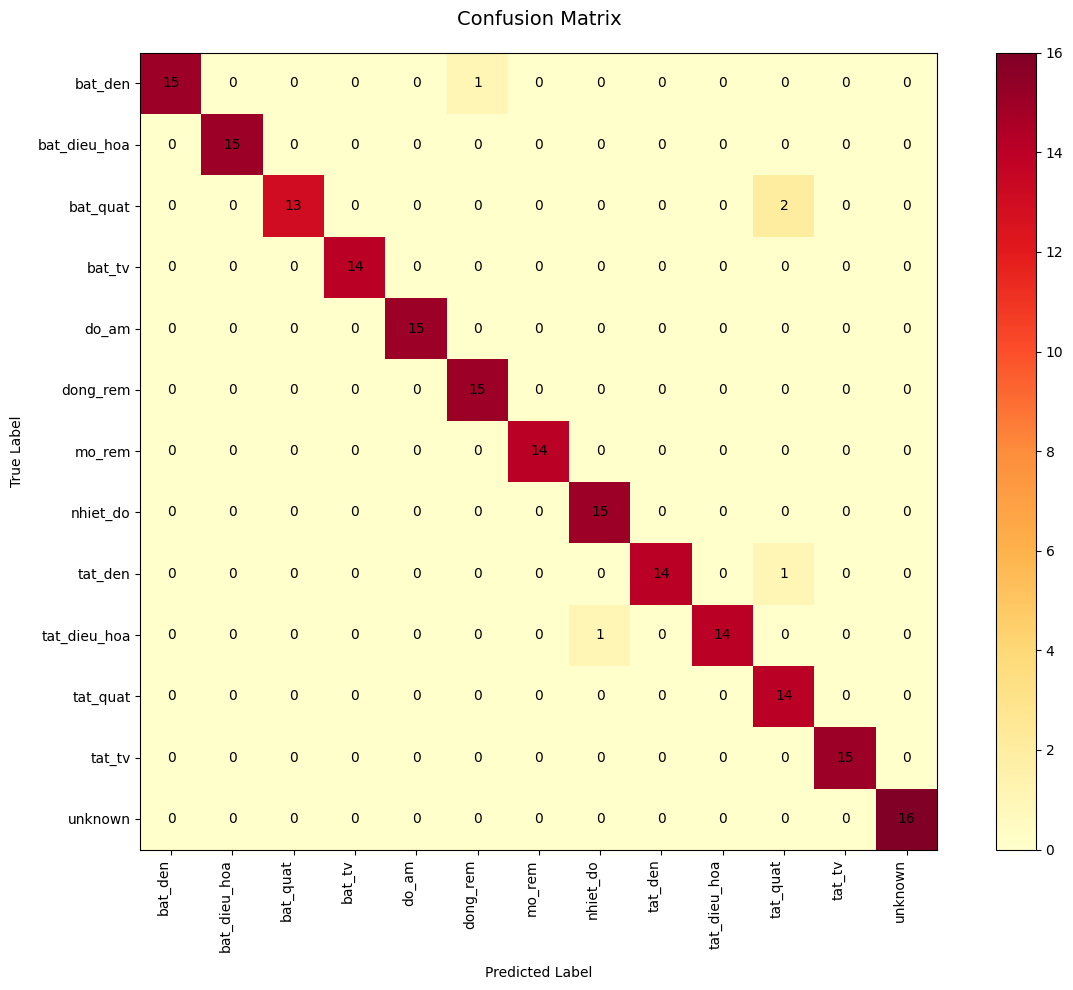
\includegraphics[width=0.75\linewidth]{imgs/fig6.png}

\caption{
Confusion matrix illustrating the classification performance across all 13 command classes.
Most misclassifications occur between acoustically similar commands, such as \textit{bat\_quat} and \textit{tat\_quat}
}

\label{fig:confusion}

\end{figure}

\begin{figure}[htbp]

\centering

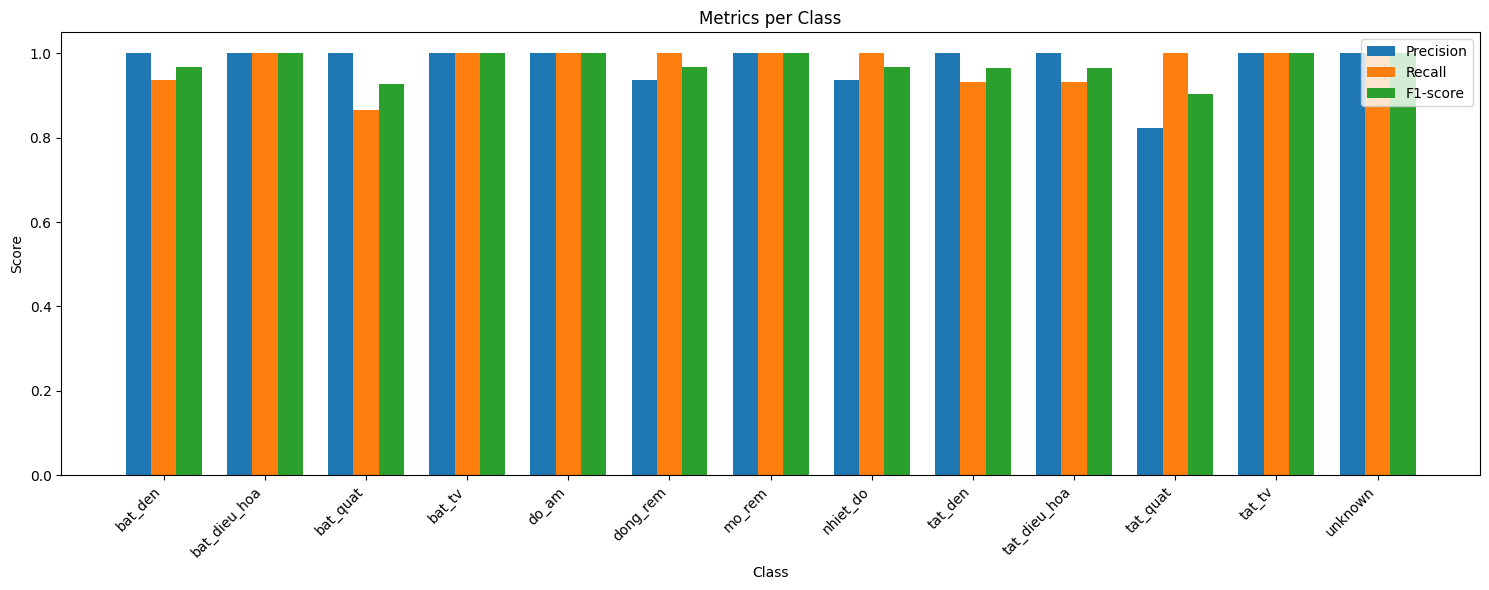
\includegraphics[width=0.8\linewidth]{imgs/fig7.png}

\caption{
Class-wise metrics (Precision, Recall, and F1-score) of the ConvMixer model,
highlighting high robustness across most classes, with slight performance dips for \textit{tat\_quat} (0.94) and \textit{bat\_quat} (0.94)
}

\label{fig:metrics}

\end{figure}

The confusion matrix in Figure~\ref{fig:confusion} confirms that classification errors primarily occur between semantically or acoustically similar commands,

while Figure~\ref{fig:metrics} presents detailed per-class performance metrics, demonstrating overall model robustness.



\subsection*{Comparative Interpretation Under Controlled Settings}

Under the revised protocol, model comparisons are now designed to be controlled and statistically grounded rather than cross-dataset or single-run. This shift allows conclusions to be framed in terms of competitiveness, parameter efficiency, and stability across seeds, instead of absolute superiority claims. In this context, ConvMixer is evaluated as a lightweight patch-based alternative whose strengths are expected to derive from depthwise spatial mixing and pointwise channel mixing under consistent Mel-spectrogram inputs.

The comparative discussion focuses on: (i) accuracy/F1 trade-offs versus parameter count, (ii) variance across seeds as a robustness indicator, and (iii) computational cost versus performance for deployment-oriented scenarios. From Table~\ref{tab:controlled_model_comparison}, ResNet-18 currently provides the highest accuracy/F1, while ConvMixer offers a substantially smaller model footprint (0.72M parameters) with competitive quality and lower runtime than heavier architectures.
